%!TEX TS-program = xelatex
\documentclass[]{friggeri-cv}
\usepackage{afterpage}
\usepackage{hyperref}
\usepackage{color}
\usepackage{xcolor}
\usepackage{smartdiagram}
\usepackage{fontspec}
% if you want to add fontawesome package
% you need to compile the tex file with LuaLaTeX
% References:
%   http://texdoc.net/texmf-dist/doc/latex/fontawesome/fontawesome.pdf
%   https://www.ctan.org/tex-archive/fonts/fontawesome?lang=en
%\usepackage{fontawesome}
\usepackage{metalogo}
\usepackage{dtklogos}
\usepackage[utf8]{inputenc}
\usepackage{tikz}
\usetikzlibrary{mindmap,shadows}
\hypersetup{
pdftitle={Alex Irmel Oviedo Solis - Ing. Informatico y de Sistemas},
pdfauthor={Ing. Alex Irmel Oviedo Solis},
pdfsubject={Curriculum vitae},
pdfkeywords={},
colorlinks=false,           % no lik border color
allbordercolors=white       % white border color for all
}
\smartdiagramset{
bubble center node font = \footnotesize,
bubble node font = \footnotesize,
% specifies the minimum size of the bubble center node
bubble center node size = 0.5cm,
%  specifies the minimum size of the bubbles
bubble node size = 0.5cm,
% specifies which is the distance among the bubble center node and the other bubbles
distance center/other bubbles = 0.3cm,
% sets the distance from the text to the border of the bubble center node
distance text center bubble = 0.5cm,
% set center bubble color
bubble center node color = pblue,
% define the list of colors usable in the diagram
set color list = {lightgray, materialcyan, orange, green, materialorange, materialteal, materialamber, materialindigo, materialgreen, materiallime},
% sets the opacity at which the bubbles are shown
bubble fill opacity = 0.6,
% sets the opacity at which the bubble text is shown
bubble text opacity = 0.5,
}

\addbibresource{bibliography.bib}
\RequirePackage{xcolor}
\definecolor{pblue}{HTML}{0395DE}

\begin{document}
\header{Alex Irmel}{Oviedo Solis}
{Ing. Inform\'atico de Sistemas}

% Fake text to add separator
\fcolorbox{white}{gray}{\parbox{\dimexpr\textwidth-2\fboxsep-2\fboxrule}{%
.....
}}

% In the aside, each new line forces a line break
\begin{aside}
    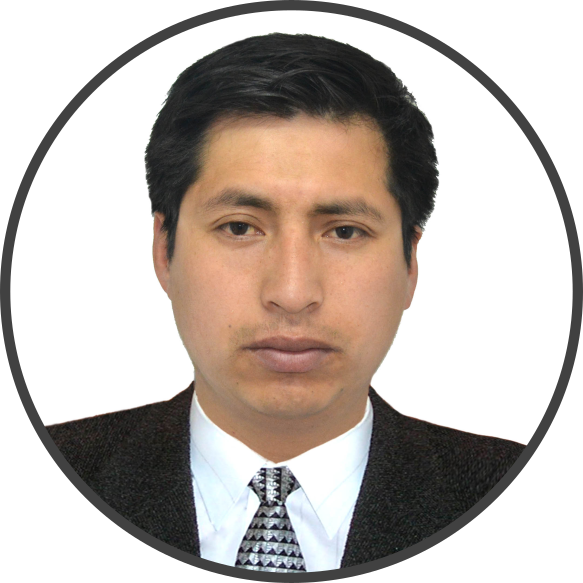
\includegraphics[scale=0.18]{img/aoviedo.png}
    \section{Direcci\'on}
    Av. de la cultura 2505
    Cusco, Cusco
    ~
    \section{Telefonos}
    +51 930 328 402
    ~
    \section{Correo electronico}
    \href{mailto:aoviedosolis@gmail.com}{\textbf{aoviedosolis@}\\gmail.com}
    \href{mailto:alexove@fedoraproject.org}{\textbf{alexove@}\\fedoraproject.org}
    ~
    \section{Web \& Git}
    \href{https://github.com/alexove}{https://github.com/alexove}
    % ~
    % % use  \hspace{} or \vspace{} to change bubble size, if needed
    % \section{Cualidades Personales}
    % \smartdiagram[bubble diagram]{
    % \textbf{Trabajo}\\\textbf{en equipo},
    % \textbf{Iniciativa},
    % \textbf{Curiosidad},
    % \textbf{Resolucion}\\\textbf{problemas},
    % \textbf{\vspace{2mm}Gerencia\vspace{2mm}},
    % \textbf{Organizado}
    % }
    ~
    \section{Idiomas}
    \textbf{Espa\~nol}
\includegraphics[scale=0.40]{img/5stars.png}
    \textbf{Ingles}
\includegraphics[scale=0.40]{img/3stars.png}
    \textbf{Ruso}
\includegraphics[scale=0.40]{img/2stars.png}
    ~
\end{aside}
~
\section{Ingeniero Inform\'atico y de Sistemas}
\emph{Con predisposici\'on para el cumplimiento de metas y objetivos, actitud pro-activa,
capacidad para trabajar en equipos multidisciplinarios, Trabajo en equipo bajo presi\'on,
capacidad de adaptaci\'on a cambios, alta confiabilidad, aspiraci\'on de desarrollo
profesional y capacidad para interactuar con personas dentro y fuera de la organizaci\'on y
deseos de progreso continuo.}
\\
\section{Educaci\'on}
\begin{entrylist}
    \entry
    {2019 - 2021}
    {Maestria en Seguridad Informatica}
    {Universidad de la Rioja - Sede Mexico}
    {Maestría enfocada en las \'ultimas t\'ecnicas de protecci\'on ante
    vulnerabilidades de sistemas operativos, software, bases de datos, sistemas
    web y todos los riesgos inherentes al empleo de las TIC y su posible repercusi\'on
    dentro de la estructura organizativa p\'ublica y privada.\\}
    \entry
    {2016 - 2017}
    {Maestria en Administraci\'on de negocios}
    {Universidad Andina del Cusco}
    {La Maestr\'ia en Administraci\'on de Negocios es un programa orientado a la formaci\'on
    profesionales de la Region Cusco y  del pa\'is, comprometi\'endolos con la realidad
    de un entorno que exige cada vez m\'as el conocimiento y el uso correcto y
    adecuado de la informaci\'on, con capacidad para responder con rigor, oportunidad
    y pertinencia social a los problemas locales, regionales y nacionales.\\}
    \entry
    {2009 - 2012}
    {Ing. Informatico y de Sistemas}
    {Universidad Nacional de San Antonio Abad del Cusco}
    {Profesional \'integro, \'etico, solidario, con s\'olida formaci\'on en la ciencias
    b\'asicas, Inform\'atica y de sistemas. Competente en el desarrollo de proyectos
    inform\'aticos, con capacidad para dise\~narlos, gerenciarlos, auditarlos y
    llevar el control y avance de los mismos.\\}
    \entry
    {2002 - 2009}
    {Bach. en Ing. Informatica y de Sistemas}
    {Universidad Nacional de San Antonio Abad del Cusco}
    {Profesional \'integro, \'etico, solidario, con s\'olida formaci\'on en la ciencias
    b\'asicas, Inform\'atica y de sistemas. Competente en el desarrollo de proyectos
    inform\'aticos, con capacidad para dise\~narlos, gerenciarlos, auditarlos y
    llevar el control y avance de los mismos.}
    \entry
    {1997 - 2001}
    {Educaci\'on Secundaria}
    {Colegio Particular Mixto Isaiah Bowman}
    {La Institucion Educativa Isaiah Bowman se creo el a\~no 1985, con 31 a\~nos de historia
    y miles de jovenes egresados de esta prestigiosa instituci\'on.}
\end{entrylist}
\\

\newpage
\begin{aside}
    ~
    ~
    \section{Lenguajes de programaci\'on}
    
\includegraphics[scale=0.20]{img/java}
    
\includegraphics[scale=0.07]{img/groovy}
    
\includegraphics[scale=0.3]{img/bash}
    ~
    ~
    \section{Preferencia de Sistema Operativo}
    \textbf{GNU/Linux}
\includegraphics[scale=0.40]{img/5stars.png}
    \textbf{Windows}
\includegraphics[scale=0.40]{img/1stars.png}
    ~
    \section{Bases de datos}
    ~
    
\includegraphics[scale=0.04]{img/mysql.png}
    
\includegraphics[scale=0.30]{img/mariadb.png}
    ~
    \section{Desarrollo web}
    ~
    
\includegraphics[scale=0.02]{img/grails.png}
    ~
\end{aside}
\section{Certificaciones}
\begin{entrylist}
    \entry
    {04/2016}
    {Linux Foundation Certified System Administrator LFCS}
    {Linux Foundation}
    {Linux Foundation certifications give you a way to differentiate yourself in
    a job market that's hungry for your skills. We've taken a new, innovative
    approach to Linux certification that allows you to showcase your skills in a
     way that other sysadmins will respect and employers will trust.\\
     \emph{Certificate ID N°{:} LFCS-1600-0744-0100}}
\end{entrylist}

\section{Experiencia}
\begin{entrylist}
    \entry
    {03/24 - 01/25}
    {Responsable de Data Center}
    {Gobierno Regional de Cusco}
    {Actividades realizadas: Responsable de Data Center (Administraci\'on de servidores GNU/Linux, supervisi\'on
    de redes), Encargado de soporte y mantenimiento de SIAF-MEF. Gobierno Digital y Seguridad de la Información.}
    \entry
    {09/23 - 02/24}
    {Desarrollador BIM}
    {Consorcio Rios del Norte S.A.C.}
    {Actividades realizadas: Planificación, desarrollo de sistma de gestión de calidad y automatización de procesos dentro 
    del marco del BIM.}
    \entry
    {12/22 - 08/23}
    {Jefe de Informatica y Sistemas}
    {MacSalud S.A.C.}
    {Actividades realizadas: Planificación, desarrollo, asignación de recursos y tareas, coordinación de proyectos de 
     sistemas de información, soporte de redes, centro de datos e Internet.}
    \entry
    {02/22 - 11/22}
    {Coordinador de proyecto de software}
    {Gerencia Regional de Educación del Cusco}
    {Actividades realizadas: Planificación, desarrollo, asignación de recursos y tareas,
     ejecución, seguimiento y entrega de Plataforma Virtual Educativa CREE.}
    \entry
    {08/21 - 09/21}
    {Analista de Seguridad de Información y Aplicaciones}
    {Caja Municipal Cusco}
    {Actividades realizadas: Monitoreo de controles de seguridad de la información. Analisis de Riesgos de Seguridad
    de la Información.}
    \entry
    {03/21 - 07/21}
    {Responsable de Data Center}
    {Gobierno Regional del Cusco}
    {Actividades realizadas: Responsable de Data Center (Administraci\'on de servidores GNU/Linux, supervisi\'on
    de redes), Encargado de soporte y mantenimiento de SIGA-MEF y SIAF.\\}
    \entry
    {01/20 - 03/21}
    {Responsable de la Oficina Funcional de Informatica}
    {Gobierno Regional del Cusco}
    {Actividades realizadas: Jefatura de la Oficina Funcional de Informatica, coordinación de proyectos de sistemas de información,
     soporte de redes, centro de datos e Internet. Parte del Comite de Gobierno Digital y Seguridad Digital.\\}
    \entry
    {01/18 - 12/19}
    {Responsable de Data Center}
    {Gobierno Regional del Cusco}
    {Actividades realizadas: Responsable de Data Center (Administraci\'on de servidores GNU/Linux, supervisi\'on
    de redes), Encargado de soporte y mantenimiento de SIGA-MEF y SIAF.\\}
    \entry
    {02/17 - 06/17}
    {Desarrollador de software GIS}
    {CEC Guaman Poma de Ayala}
    {Desarrollador de Sistema de Informaci\'on Georeferenciado utilizando java con gvSIG y PostgreSQL.\\}
\end{entrylist}
\begin{entrylist}
    \entry
    {04/16 - 07/16}
    {Responsable de Data Center}
    {Gobierno Regional del Cusco}
    {Actividades realizadas: Responsable de Data Center (Administraci\'on de servidores GNU/Linux, supervisi\'on
    de redes), Encargado de soporte y mantenimiento de SIGA-MEF y SIAF.\\}
    \entry
    {02/16 - 03/16}
    {Docente de Ofim\'atica}
    {CENFOTI – Universidad Andina del Cusco.}
    {Actividades realizadas: Docente de Ofim\'atica.\\}
    \entry
    {07/15 - 12/15}
    {Responsable de Data Center}
    {Gobierno Regional del Cusco}
    {Responsable de Data Center (Administraci\'on de servidores GNU/Linux, supervisi\'on de redes), Encargado de
    soporte y mantenimiento de SIGA-MEF.\\}
    \entry
    {01/15 - 03/15}
    {Responsable de Data Center}
    {Gobierno Regional del Cusco}
    {Responsable de Data Center (Administraci\'on de servidores GNU/Linux, supervisi\'on de redes), Encargado de
    soporte y mantenimiento de SIGA-MEF.\\}
    \entry
    {06/14 - 10/14}
    {Desarrollador de software}
    {Las Bambas - ManPower}
    {Desarrollador de aplicaciones web para mina (sistema de informaci\'on para perforaciones y voladuras).\\}
    \entry
    {07/12 - 02/14}
    {Desarrollador Web con Java}
    {Java For Smart Information Technologies - Cusco}
    {Desarrollador Web con Java, JSP. GWT b\'asico, Desarrollo de Android Intermedio, Framework GRAILS, Administraci\'on de Servidores virtuales.\\}
    \entry
    {11/12 - 01/13}
    {Responsable de Data Center}
    {{RootWay Internet Services \& Consulting - Uruguay}}
    {{Administraci\'on y migraci\'on de servidores virtuales, GNU/Linux en AmazonWS. \\ }}
    \entry
    {01/12 - 05/12}
    {Jefe de la Oficina de Inform\'atica.}
    {Municipalidad Provincial de Quispicanchi}
    {Jefe de la Oficina de Inform\'atica.\\}
\end{entrylist}
\begin{aside}
    ~
    \section{GNU/Linux}
    ~
    
\includegraphics[scale=0.12]{img/fedora}
    
\includegraphics[scale=0.12]{img/centos}
    ~
\end{aside}
\section {Diplomados}
\begin{entrylist}
  \entry
  {10/2020 - 03/2021}
  {Gestión de la Seguridad y Marco Legal}
  {Universidad Internacional de la Riona en México}
  {Realizado del 26 de octubre de 2020 al 7 de marzo de 2021, con una duración de 432 horas}
  \entry
  {05/2020 - 08/2020}
  {Seguridad en los Nuevos Entornos y Auditoría}
  {Universidad Internacional de la Riona en México}
  {Realizado del 4 de mayo de 2020 al 30 de agosto de 2020, con una duración de 360 horas}
  \entry
  {10/2019 - 03/2020}
  {Seguridad en Redes, Sistemas y Aplicaciones}
  {Universidad Internacional de la Riona en México}
  {Realizado del 28 de octubre de 2019 al 8 de marzo de 2020, con una duración de 360 horas}
\end{entrylist}
\newpage
\section{Cursos y seminarios}
\begin{entrylist}
    \entry
    {01/25 - 01/25}
    {Arquitectura de Software en la Práctica}
    {UDEMY}
    {Curso dictado por Likecomtic - Arquitectura de Software durante 12 horas cronologicas.\\}
    \entry
    {12/24 - 12/24}
    {Gestión por Procesos e Inteligencia Artificial}
    {GFP Subnacional}
    {Seminario ofrecido por el Programa GFP Subnacional de la Cooperación Suiza-SECO por 4 horas lectivas.\\}
    \entry
    {09/24 - 09/24}
    {Transformación Digital en el Perú}
    {ENAP}
    {Curso ofrecido por la Escuela Nacional de Administración Pública por 24 horas lectivas.\\}
    \entry
    {08/24 - 08/24}
    {Plataforma Digital de Gestión Documental Cero Papel}
    {SGTD-PCM}
    {Seminario ofrecido por la Secretaría de Gobierno y Transformación Digital de la PCM.\\}
    \entry
    {05/24-05/24}
    {Gestión de Proyectos de Inversión Pública en el Marco del INVIERTE.PE}
    {ENCAP}
    {Curso ofrecido por Escuela Nacional de Capacitación y Actualización Profesional por 60 horas academicas.\\}
    \entry
    {08/23 - 08/23}
    {Habilidades Gerenciales para el Pequeño Empresario}
    {UDEMY}
    {Curso dictado por Tomas Bradanovic durante 2 horas lectivas.\\}
    \entry
    {01/23 - 01/23}
    {Asterisk nativo, configura tu Central Telefonica desde cero}
    {UDEMY}
    {Curso dictado por Roger Mamani durante 11 horas lectivas.\\}
    \entry
    {01/23 - 01/23}
    {Gestión de riesgos ISO/IEC 27005, con formatos editables}
    {UDEMY}
    {Curso dictado por Israel Rogelio Gomez durante 2 horas lectivas.\\}
    \entry
    {01/23 - 01/23}
    {ISO/IEC 27001 Implementando Seguridad de la Información}
    {UDEMY}
    {Curso dictado por Grover Vasquez durante 2 horas lectivas.\\}
    \entry
    {11/21 - 11/21}
    {Diseño y construcción de redes de fibra optica}
    {UDEMY}
    {Curso ofrecido por Gaston Fenske durante 2.5 horas lectivas.\\}
    \entry
    {08/21 - 08/21}
    {Analisis de Vulnerabilidades Digitales}
    {Centro Nacional de Seguridad Digital}
    {Curso ofrecido por el Centro Nacional de Seguridad Digital (PCM-SEGDI) durante 24 horas lectivas.\\}
    \entry
    {06/21 - 06/21}
    {Auditor Interno ISO 27001}
    {Centro Nacional de Seguridad Digital}
    {Curso ofrecido por el Centro Nacional de Seguridad Digital (PCM-SEGDI) durante 24 horas lectivas.\\}
    \entry
    {05/21 - 05/21}
    {Linux Essentials}
    {Centro Nacional de Seguridad Digital}
    {Curso ofrecido por el Centro Nacional de Seguridad Digital (PCM-SEGDI) durante 24 horas lectivas.\\}
\end{entrylist}
\begin{entrylist}
    \entry
    {04/21 - 04/21}
    {SCRUM Práctico en Proyectos de Software}
    {UDEMY}
    {Curso dictado por Hector Bravo durante 4.5 horas lectivas.\\}
    \entry
    {10/18 - 10/18}
    {Curso PRE-MTCNA Mikrotik}
    {COMUTEL}
    {Curso dictado por COMUTEL durante 16 horas lectivas.\\}
    \entry
    {12/15 - 01/16}
    {Curso OFICIAL ITIL FOUNDATION}
    {BSGrupo}
    {Realizado entre el 06 de diciembre del 2015 y el 06 de enero del 2016.\\}
\end{entrylist}

\section{Congresos y ponencias}
\begin{entrylist}
  \entry
    {11/2016}
    {\textbf{Ponente} VI Encuentro de Ing. de Sistemas e Inform\'atica }
    {UTEA}
    {Realizado del 16 al 18 de noviembre del 2015 en la Universidad Tecnológica de los Andes - Sede Cusco.\\}
\end{entrylist}
\begin{entrylist}
    \entry
    {09/2015}
    {\textbf{Ponente} Fedora Users and Developers Conference - Argentina}
    {Fedora Community}
    {Realizando en la ciudad de Cordoba-Argentina, entre 10 y 12 de septiembre
    del 2015 en la Universidad Nacional de C\'ordoba – Argentina.\\}
    \entry
    {08/2015}
    {\textbf{Ponente} {XXIII CONEISC}}
    {Universidad Catolica Santa Maria}
    {Realizado entre el 17 al 21 de agosto del 2015 en la Universidad Catolica Santa Maria, Arequipa, Peru.\\}
    \entry
    {11/2014}
    {\textbf{Ponente} VI Festival Internacional de Software Libre SOFLISEOANE}
    {Instituto de Educaci\'on Superior Tecnol\'ogico Publico Manuel Seoane Corrales}
    {Realizado el 28 y 29 de noviembre del 2014 en el Instituto de Educaci\'on Superior
    Tecnol\'ogico Publico Manuel Seoane Corrales, Lima.\\}
    \entry
    {04/2014}
    {\textbf{Ponente} 15-vo Foro Internacional do Software Livre-Porto Alegre-Brasil}
    {FISL}
    {Realizado entre el 7 y 10 de mayo del 2014 en la ciudad de Porto Alegre-Brasil.\\}
    \entry
    {01/14 - 03/14}
    {Curso Taller de "SEGURIDAD INFORM\'ATICA"}
    {Grupo Development In Peru SCRL}
    {Organizado por el Grupo Development In Peru SCRL.\\}
    \entry
    {12/2015}
    {\textbf{Ponente} Semana Informatica INSANE CODE}
    {IST Tupac Amaru}
    {Organizado por el Instituto de Educaci\'on Superior Tecnol\'ogico Publico "Tupac
    Amaru" del Cusco.}
\end{entrylist}
\begin{entrylist}
    \entry
    {10-2013}
    {\textbf{Ponente} IV ENCUENTRO DE INGENIERIA DE SISTEMAS E INFORMATICA}
    {UTEA}
    {Realizado los d\'ias 26 y 27 de octubre del 2013 organizado por la Universidad
    Tecnol\'ogica de los Andes.\\}
    \entry
    {09-2012}
    {Encuentro GOOGLE DEVELOPMENT FEST LIMA}
    {Google Developers Group}
    {Realizado el 27 y 28 de octubre del 2012 y organizado por Google Developer Group Lima.},
    \entry
    {08-2012}
    {Seminario Taller de Regional ESTRATEGIA NACIONAL DE GOBIERNO ELECTRONICO}
    {ONGEI}
    {Realizado el 13 y 14 de septiembre del 2012, organizado por la Oficina
    Nacional de Gobierno Electr\'onico e Inform\'atica.}
\end{entrylist}
%
%\begin{flushleft}
%    \emph{May 8th, 2016}
%\end{flushleft}
%\begin{flushright}
%    \emph{John Snow}
%\end{flushright}

\end{document}
